\chapter{Desenvolvimento} \label{desenvolvimento}

Antes de iniciar o desenvolvimento, foi realizada uma extensa pesquisa sobre missões com \textit{CubeSats} para buscar referências e teve por objetivo entender os requisitos e especificações de outras missões bem sucedidas e usar essas informações como um guia para o EPS que será desenvolvido no LODESTAR. 

A tabela \ref{history_table} mostra as missões, ano de deploy e um resumo das soluções utilizadas.

\begin{table}
\centering
\caption{Missões anteriores com \textit{Cubesats}}
\label{history_table}
\begin{tabular}{|l|l|l|l|} 
\hline
\multicolumn{1}{|c|}{Nome} & \multicolumn{1}{c|}{Tipo} & \multicolumn{1}{c|}{Ano} & \multicolumn{1}{c|}{Implementação do EPS}  \\ 
\hline
Cute 1.7+                  & Demonstração              & 2008                     &  Implementação do MPPT, centralizado  \\ 
\hline
SNAP-1                     & Demonstração              & 2000                     &  Implementação do MPPT, parcialmente distribuído  \\
\hline
ESTCube-1                  & Científico                & 2013                     &  Controladores MPPT, centralizado     \\ 
\hline
SwissCube                  & Observação                & 2009                     &  Implementação do MPPT, centralizado  \\
\hline
\end{tabular}
\end{table}

O CUTE \cite{cute1_ref} (Cubical  Tóquio  Tech  Engineering  Satellite-I) é um projeto cooperativo do LSS (Laboratory for Space Systems) e o SRTL (Space Robotics and Teleoperations Laboratory), ambos de Tóquio. O EPS utilizava 4 baterias de Li-ion e as células solares proviam em média 4 W, possuia linhas estabilizadas de 3.3, 5, 6 e 7 V. O  projeto  educacional  de  baixo  custo  usava componentes COTS para uma missão de demonstração tecnológica, o projeto teve outros lançamentos posteriores. (Cute-I, Cute 1.7+ APD, Cute 1.7+ APD II). 

O SNAP-1 \cite{snap1_ref} foi o primeiro nanossatélite desenvolvido no Reino Unido pela Surrey Space Centre (SSC) e Surrey Satellite Tecnology Ltd (SSTL) e serviu como veículo de teste para demonstração da nova tecnologia que estava surgindo, ele foi um dos pioneiros dessa nova filósofia de design e mostrou que era possível construir um nanossatélite rapidamente e com custo baixo, utilizando peças COTS. O seu EPS tem uma arquitetura parcialmente distribuida, porque das suas duas linhas de tensão (5 e 12 V), a de 12 V não é regulada, dessa forma, cada módulo que utilize essa linha deve implementar a regulação. Além disso, utiliza uma única bateria de 10 Wh e o EPS tem um modo burst, onde é possível utilizar até 60 W por alguns minutos.

ESTCube-1 \cite{estcube1_ref} foi um \textit{cubesat} 1U lançado pelo foguete Vega VV02. Desenvolvido por uma força tarefa de 4 universidades, tinha o objetivo científico de realizar um prova de conceito de medição e demonstração da tecnologia da tecnologia de velas solares elétricas. O seu EPS utilizava um design próprio um controlador MPPT da STMicroelectronics (SPV1040) para cada 4 células solares com duas baterias 18650 da Panasonic totalizando 9 Wh e linhas controladas de 12, 5 e 3.3 V.

O SwissCube-1, \cite{swisscube_ref}\cite{lessons_swisscube_ref} foi um \textit{cubesat} suíço científico de tamanho 1U, operado pela Ecole Polytechnique Fédérale de Lausanne (EPFL) para realizar pesquisas sobre o \textit{nightglow} (fenômeno de brilho noturno na atmosfera terrestre) e também para desenvolver tecnologia para futuras naves espaciais. O seu EPS utilizava um design próprio com duas baterias de 1200 mAh, uma única linha de tensão, controlada por um circuito analógico, de 3.3 V,  e possui um sistema de beacon integrado que funciona sem o auxilio de microcontroladores externos, como os do OBC, por exemplo.

\section{Análise de consumo energético da missão}

Um dos pontos centrais para um projeto de EPS é dimensionar o \textit{payload} e os outros subsistemas para o pior cenário de consumo. O EPS deve ser capaz de manter o \textit{cubesat} em funcionamento quando esse cenário estiver presente. A tabela \ref{tab:requisites_modules} mostra os consumos máximos absolutos separados por módulo.

\begin{table}[!ht]
    \centering
    \begin{tabular}{l|ccc}
        Subsistema & Corrente & Tensão & Potência \\
        \hline
        Atuador magnético & \SI{900}{\milli\ampere} & \SI{5}{\volt} & \SI{4,5}{\watt}\\
        On board computer (OBC) & \SI{160}{\milli\ampere} & \SI{5}{\volt} & \SI{0.8}{\watt}\\
        Transceiver UHF & \SI{1.2}{\ampere} & \SI{3.3}{\volt} & \SI{3.96}{\watt}\\
        AD\&CS & \SI{2}{\milli\ampere} & \SI{3.3}{\volt} & \SI{6.6}{\milli\watt}\\
        \hline
        Total \SI{3.3}{\volt} & ~\SI{1.202}{\ampere} & - & \SI{3.9666}{\watt}\\
        Total \SI{5}{\volt} & ~\SI{1.06}{\ampere} & - & \SI{5.3}{\watt}\\ \hline
        Total & ~\SI{2.46}{\ampere} & - & \SI{9.26}{\watt}\\
    \end{tabular}
    \caption{Requisitos de potência para cada subsistema}
    \label{tab:requisites_modules}
\end{table}

A pesquisa pelos outros EPSs lançados nos mostrou algumas opções com relação a arquitetura. A primeira decisão é sobre quem é responsável por fazer a regulação e distribuição das linhas, ou seja, se o EPS deve centralizar a regulação das linhas e já fornecer a alimentação para os diversos módulos já com a tensão e carga requeridas por cada um deles. A outra opção é distribuir essa responsabilidade entre os módulos de forma que cada é responsável por regular as tensões necessárias para o funcionamento interno daquele módulo. Usualmente, quando o EPS é responsável pela regulação das linhas de tensão existe também alguma interface que permita aos módulos controlar qual linha está ligada em um dado momento, normalmente o protocolo $I^{2}C$ é o escolhido para essa comunicação.

A segunda decisão arquitetural envolve a implementação da técnica MPPT, que será utilizada para maximizar a eficiência do painel solar, em uma das arquiteturas as células solares são colocadas em regime MPPT com um conversor DC/DC, um microcontrolador é usado para ajustar o \textit{Duty Cycle} de uma \textit{PWM - Pulse Width Modulation} e colocar esse ponto baseado na tensão e corrente da célula solar. A saída do conversor DC/DC é conectada a um circuito de proteção da bateria, responsável por parar o carregamento caso esta esteja totalmente carregada. Esse módulo também é responsável pela proteções de subtensão e sobrecorrente, o que consiste em basicamente desligar as cargas para proteger a saúde da bateria, dado que existe um limite até é possível que ela seja descarregada. A outra opção existente é utilizar um controlador MPPT completo, onde toda essa funcionalidade está integrada em um único chip.

Após isso, a saída protegida é regulada para multiplas linhas que podem alimentar um ou mais subsistemas. 

Baseado nessa arquitetura e nas especificações do padrão Cubesat, a figura \ref{fig:block_diagram} mostra o diagrama de blocos da implementação proposta:

\noindent
\begin{minipage}{\linewidth}
\makebox[\linewidth]{
    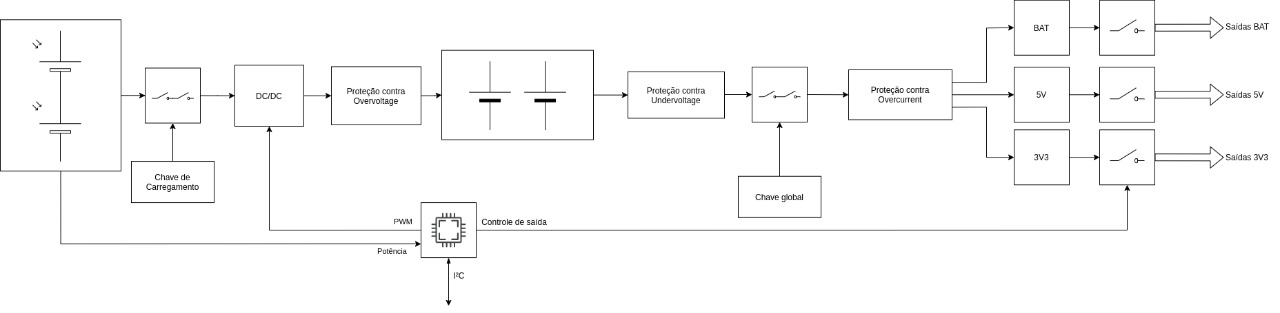
\includegraphics[angle=270,keepaspectratio=true, scale=0.55]{imagens/DiagramaBlocos.jpeg}}
\captionof{figure}{Diagrama de blocos proposto para o EPS}
\label{fig:block_diagram}
\end{minipage}

Com essa arquitetura definida, o trabalho de pesquisa e simulação dos componentes foi dividido entre eu e outro aluno do laboratório LODESTAR, Luiz Antônio, que está trabalhando com a parte da regulação das linhas de tensão a partir da bateria, dessa forma estamos abarcando todos os requisitos propostos inicialmente para o EPS.

\subsection*{Tarefas e \textit{Power Budget}}

Após levantar os consumos de cada módulo, o próximo passo é construir um \textit{power budget} baseado nas tarefas que o \textit{cubesat} precisa realizar ao longo de um ciclo.  

Alguns blocos da figura \ref{fig:block_diagram}, tais como as células solares e baterias foram escolhidas baseadas no \textit{power budget} disponível. Segue abaixo o \textit{power budget} estimado para a missão, detalhando cada um dos componentes e seus consumos, baseado nisso, e usando as informações da órbita, é possível determinar o número minímo de baterias e de células solares para conseguir carregar com sucesso o conjunto de baterias durante um ciclo. A figura \ref{fig:power_budget} mostra o \textit{power budget}:

\noindent
\begin{minipage}{\linewidth}
\makebox[\linewidth]{
    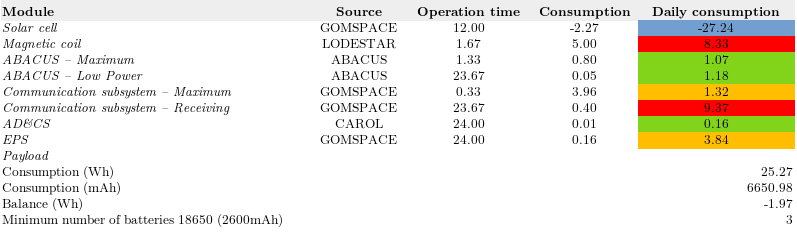
\includegraphics[keepaspectratio=true, scale=0.5]{imagens/powerbudget.png}}
\captionof{figure}{\textit{Power budget} estimado para o EPS}
\label{fig:power_budget}
\end{minipage}

As seguintes premissas foram consideradas na construção dessa tabela:

\begin{enumerate}
    \item O sistema de comunicação irá operar por um período máximo de 20 minutos e permanecerá em modo de recepção durante o restante do ciclo.
    \item O consumo do atuador magnético está modelado para funcionar com pulsos de 1 minuto em potência máxima, é assumido que haverão 100 pulsos durante o ciclo.
    \item O computador de bordo (OBC) estará em modo ativo por no máximo 1 hora e durante o tempo que estiver ocorrendo transmissões, no total de 1 hora e 20 minutos.
    \item Apenas uma das faces do nanossatélite está exposta à radiação solar por vez.
\end{enumerate}


Na coluna \textit{Source} é colocado de onde é vieram as informações a respeito do módulo, onde aparece a GOMSpace é uma fabricante e fornecedora de nanossatélites e componentes em vários mercados, além de ser uma empresa referência no mercado, com vários cases de sucesso, o laboratório LODESTAR tem intenção de compra com a GOMSpace do nanossatélite do primeiro lançamento da missão. O Abacus é um computador de bordo (OBC) fabricado pela Gauss Srl e utilizado para testes no LODESTAR, por ser um OBC multi-propósito ele tem um consumo maior do que os computadores da GOMSpace, o que pode vir a aumentar o nosso saldo no Power Budget. O atuador magnético \cite{unb_mag_actuator} e o ADCS \cite{carol_adcs} utilizados de referência são de trabalhos desenvolvidos por alunos do laboratório. 


Com esse \textit{power budget}, a menor célular solar (1U) da GOMSPACE é usada como referência. Essa célula solar é capaz de prover até \SI{27}{\watt}. Note que usada apenas essa célula, o \textit{budget} ainda fica com um saldo negativo, o que significa que estamos consumindo menos energia do que a que conseguimos adquirir, porém essa margem ainda é pequena. Portanto, mais células solares devem ser usadas para prover uma quantidade segura de energia.

Conhecer os consumos dos módulos permitiu calcular quantas baterias, aqui estamos utilzando os modelos 18650 como referência, para manter o nanossatelite alimentado durante um ciclo. Os modelos de baterias 18650 são largamente utilizados nos EPS pela padronização de tamanho e segurança. No modelo referência da GOMSpace temos \SI{2600}{\milli\ampere\hour}, ou seja, para conseguir suprir o consumo de \SI{6650}{\milli\ampere\hour}, pelo menos três dessas baterias.

\section{Circuito de carga da bateria}

Uma das tarefas cruciais para o projeto do circuito de carga da bateria é escolher o conversor DC/DC que fará a interface entre o painel solar e a bateria, o que nos permite aplicar a técnica de MPPT. Para cumprir essa tarefa, foi realizada uma busca pelos conversores disponíveis comercialmente e na seção de resultados apresentaremos os resultados e as métricas utilizadas para escolha. 

Além do conversor DC/DC, para completar um circuito minímo para implementar o MPPT, precisamos ainda definir um microcontrolador e de algum circuito capaz de sensoriar a tensão e corrente extraída da bateria. Para esses componentes, existiram dificuldades no campo da simulação, pois não encontramos nenhum simulador que seja capaz de fazer uma simulação hibrída entre circuitos analógicos e digitais. Nesse ponto, o modelo SPICE, que é voltado para a simulação de circuitos analógicos, trouxe uma limitação muito grande, pois os microcontroladores são circuitos integrados bastante complexos, com diversas interfaces, o que impossibilita a construção de um modelo SPICE para esses chips.


\section{Solução com controlador integrado}

O uso de um chip independente para a implentação do MPPT traz muitas vantagens com relação a implementação tradicional com componentes discretos. A primeira delas é que isso torna o sistema MPPT complementamente autônomo, isso permite que o aquisição de energia continue mesmo com o esgotamento total das baterias. A segunda é por dispensar recursos do microcontrolador, seja por livrar recursos de algum que desempenha várias funcionalidade ou dispensar um microcontrolador exclusivo para essa tarefa. A terceira está relacionada com a segunda, que é o \textit{footprint} bem reduzido no projeto final da PCB, pois estamos dispensando vários componentes discretos. Para esses controladores, o problema da ausência de modelos SPICE se repete, da mesma forma que ocorreu com os microcontroladores.




